\documentclass[aspectratio=1610]{beamer}
\usepackage{iftex}
\usepackage{pdfpages}
\ifLuaTeX\else
	\usepackage[utf8]{inputenc}
	\usepackage[T1]{fontenc}
\fi
%%%%%%%
% \usepackage{layout}
% \usepackage{lipsum}
%%%%%%%
\usetheme[% Complete settings. Default value in []
% titleimagecolor=red,       % [gray], darkgray, red, blue, green
% titleimagemargin=2mm,      % Distance [2mm]    Frame around title page image
% navigationsymbols=false,   % true   / [false]  Navigation symbols in the foot
% mathseriffont=false,       % true   / [false]  Serif / non-serif math fonts
% foot=true,                 % [true] / false    Footline or not
% nofootslidenum=false       % true   / [false]  Keep slide num even when foot=false
% footlogo=true,             % [true] / false    Put LU logo to the left of footer
% english=true,              % [true] / false    English / Swedish logo
% LTHlogo=false,             % true   / [false]  Use LTH logo instead of LU on title and end pages.
% blackenumeratenumber=true, % [true] / false    Black enumerate numbers, o.w. Lund bronze
% blackitemmark=false,       % true   / [false]  Black item marks, o.w. Lund bronze
% defaultfont=palatino,      % [palatino], beamer, lu
% sectionframe=true,
]{ulund}
%%%%%%%%%%%%%%%%%%%%% Layout commands 
%%%% Foot
% \ulundfootleft{\insertshortauthor}
% \ulundfootmid{\insertshorttitle}
% \ulundfootright{\insertframenumber}% {\insertframenumber:\inserttotalframenumber}
%%%% Titleimage
% \titleimage{Pictures/ULUNDcolor} % Replaces the LU image. Voids option titleimagecolor
%%%%%%%%%%%%%%%%%%%%%%%%%%%%%%%%%%%
\title[ulund beamer]{Test of ulund beamer template}
\author[S. Höst]{%
  Stefan Höst\newline
  Dept.\@ of EIT, Lund University}
%%%%%%%%%%%%%%%%%%%%%
%\usepackage{verbatim}
%%%%%%%%%%%%% Verbatim code box
\usepackage[skins,listings]{tcolorbox}
\ifLuaTeX\else
	\tcbuselibrary{listingsutf8}
\fi
\lstdefinestyle{CodeStyle}{basicstyle = \ttfamily}
\newtcblisting{CodeBox}[2][]{% Only code
  colframe=black,
  colback=white,
  arc=1pt,
  boxrule=0.5pt,
  top=0mm,bottom=0pt,left=0pt,
  colbacktitle=gray!40,
  coltitle=black,
  fonttitle=\sffamily,
  listing only,
  title=#2,#1}
%%%%%%%%%%%%%%%%%%%%%
%%%%%%%%%%%%%%%%%%%%%
%%%%%%%%%%%%%%%%%%%%%
\begin{document}
\begin{frame}[plain]% Use plain to suppress footline box
  \titlepage
\end{frame}

%%%%%%%%%%%%%%%
\begin{frame}
  \frametitle{Beamer template: ulund}
  This file is a short introduction to the beamer template \texttt{ulund}, an attempt to mimic Lund University's ppt template in \LaTeX\ beamer.

Below follows:
\begin{itemize}
\item A short introduction to the implemented options in the template. 
\item Some examples
%\item Contact information for bug report
\end{itemize}

/Stefan Höst
\end{frame}


%%%%%%%%%%%%%%%
\section{Short manual}

%%%%%%%%%%%%%%%%
\begin{frame}[fragile]{Beamer template: ulund}
  Start by including the beamer template \verb|ulund|. The preamble for this document is essentially: 
\begin{CodeBox}{}
\documentclass[aspectratio=1610]{beamer}
\usepackage[utf8]{inputenc}
\usepackage[T1]{fontenc}
\usetheme{ulund}
\title[ulund beamer]{Test of ulund beamer template}
\author[S. Höst]{%
  Stefan Höst\newline
  Dept.\@ of EIT, Lund University}
\begin{document}
\end{CodeBox}
\end{frame}

%%%%%%%%%%%%%%%%
\begin{frame}[fragile]{LuaLaTeX support}
	If you wish to use LuaLaTeX, for example to be able to use the university profile fonts, use the following preamble, and then compile the document with \texttt{lualatex}:
\begin{CodeBox}{}
\documentclass[aspectratio=1610]{beamer}
\usetheme[defaultfont=lu]{ulund}
\title[ulund beamer]{Test of ulund beamer template}
\author[L. Karlsson]{%
Linus Karlsson\newline
Lund University}
\begin{document}
\end{CodeBox}
Also, see the \texttt{defaultfont} option described below to see important information about font selection.
\end{frame}

%%%%%%%%%%%%%%%
\begin{frame}[fragile]
  \frametitle{Options}
  The ulund theme comes with some options, as a comma separated list, set with
  \verb|\usetheme[<options>]{ulund}|.\newline
  The options are (default value in [.]):
  \begin{itemize}
  \item \verb|titleimagecolor={[gray], darkgray, red, blue, green}|\newline
    Background color of the title frame.
  \item \verb|titleimagemargin=<distance>| \newline
    White frame around title page page, default 2 mm. (Keep it $\leq 4$ mm.)
  \item \verb|navigationsymbols={true, [false]}|\newline
    Navigation symbols in the footer.
  \item \verb|mathseriffont={true, [false]}|\newline
    Serif math fonts
  \end{itemize}
\end{frame}

%%%%%%%%%%%%%%%
\begin{frame}[fragile]
  \frametitle{Options (cont'd)}
  \begin{itemize}
  \item \verb|foot={[true], false}|\newline
    Print footer.
  \item \verb|footlogo={[true], false}|\newline
    Print small LU logo to right of footer.
  \item \verb|english={[true], false}|\newline
    English LU logo. otherwise Swedish.
  \item \verb|LTHlogo={true, [false]}|\newline
    Use LTH logo on front and end page, otherwise LU (only seal)
  \end{itemize}
\end{frame}

%%%%%%%%%%%%%%%
\begin{frame}[fragile]
  \frametitle{Options (cont'd)}
  \begin{itemize}
  \item \verb|blackenumeratenumber={[true], false}|\newline
    Black enumerate numbers, otherwise Lund bronze.
  \item \verb|blackitemmark={true, [false]}|\newline
    Black item marks, otherwise Lund bronze
  \item \verb|sectionframe={[true], false}|\newline
    Print section frame for each section. Color set by \verb|titleimagecolor|.
  \end{itemize}
\end{frame}

%%%%%%%%%%%%%%%
\begin{frame}
	\frametitle{Options (cont'd)}
	\begin{itemize}
		\item \texttt{defaultfont=\{[palatino], beamer, lu\}}\newline
		Selects the default font to use. The validity of options depend on the compiler used for the \LaTeX{} document as follows:
		\begin{itemize}
			\item \texttt{palatino}\newline
			Use Palatino for titles, Helvetica as sans-serif, and Courier for monospaced text. Can be used with all compilers.
			\item \texttt{beamer}\newline
			Use the default fonts of Beamer. Can be used with all compilers.
			\item \texttt{lu}\newline
			Use the Lund University profile fonts: Adobe Garamond Pro as serif font, and Frutiger Std as sans-serif. Requires LuaLaTeX, \emph{and} the fonts to be installed on your computer. Fonts can be downloaded from: \url{https://www.staff.lu.se/support-and-tools/communication-and-graphic-profile/download-templates-and-communication-tools}
		\end{itemize}
		See the following three pages for examples of how the different fonts look.
	\end{itemize}
\end{frame}

%%%%%%%%%%%%%%%
{
	\setbeamercolor{background canvas}{bg=}
	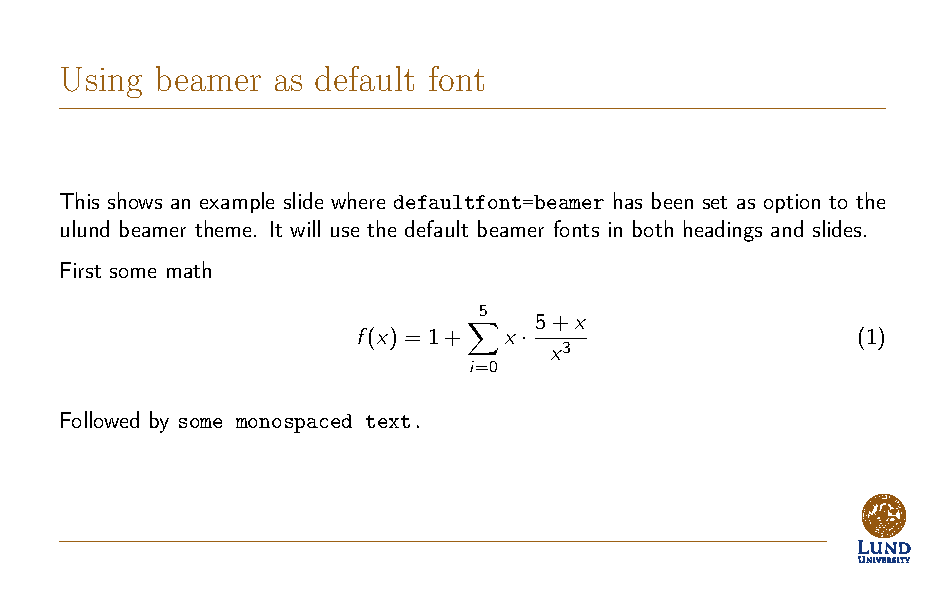
\includepdf[pages=1]{page-beamer.pdf}
}

%%%%%%%%%%%%%%%
{
	\setbeamercolor{background canvas}{bg=}
	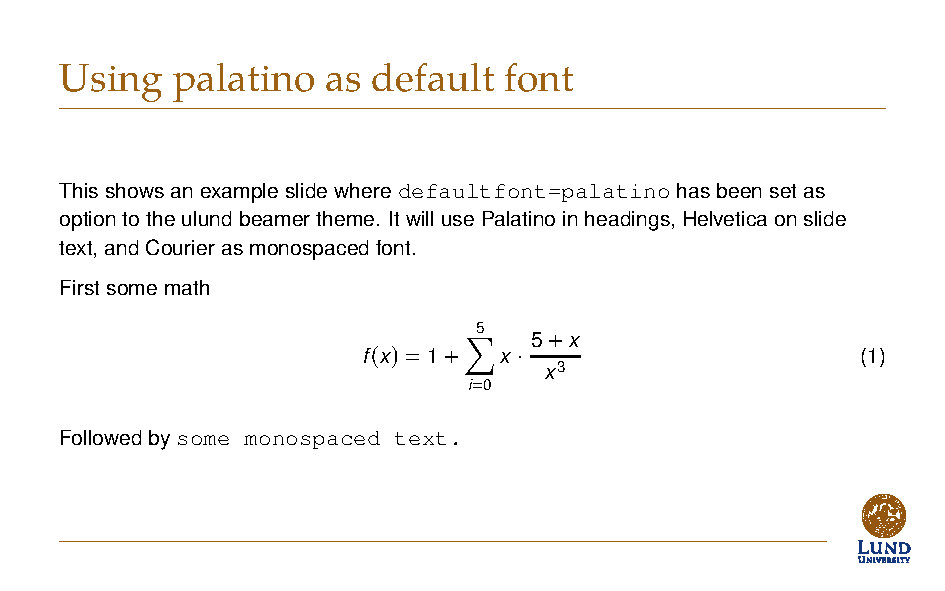
\includepdf[pages=1]{page-palatino.pdf}
}

%%%%%%%%%%%%%%%
{
	\setbeamercolor{background canvas}{bg=}
	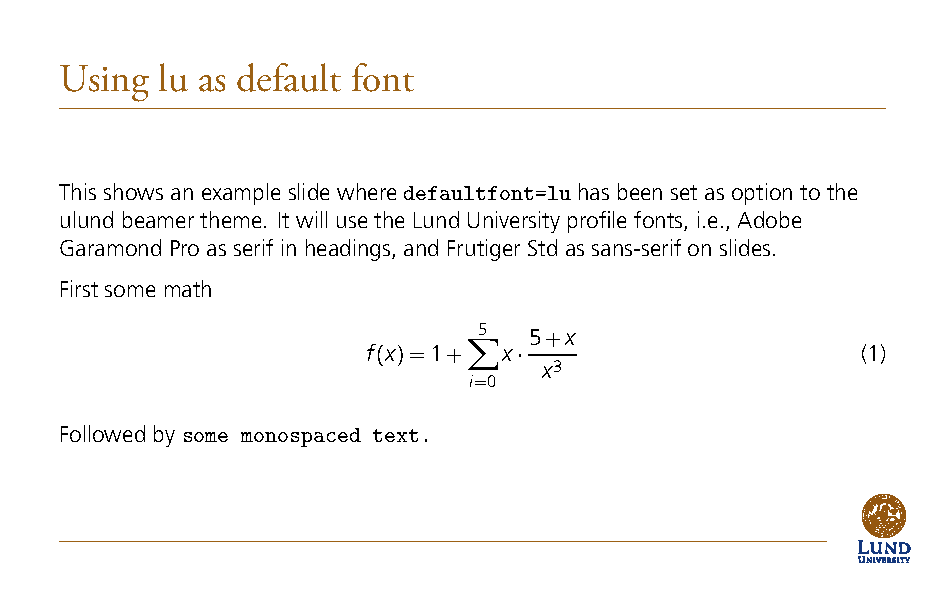
\includepdf[pages=1]{page-lu.pdf}
}

%%%%%%%%%%%%%%%
\begin{frame}[fragile]{Footer}
  In the foot there are three positions; left, mid and right. The default is
  \par\strut\par
  \rule{2em}{0pt}%
  \begin{tikzpicture}
    \draw[thin,color=lundbronze] (0,0) -- (12,0)
    node[pos=0,anchor=north west,inner sep=0pt,yshift=-5pt,black]{\texttt{<short author>}}
    node[pos=0.5,anchor=north,inner sep=0pt,yshift=-5pt,black]{\texttt{<short title>}}
    node[pos=1,anchor=north east,inner sep=0pt,yshift=-5pt,black]{\texttt{<frame number>}};
  \end{tikzpicture}
  \par\strut\par
  To set some other content in the foot use the commands (here with default value)
  \begin{itemize}
  \item \verb|\ulundfootleft{\insertshortauthor}|
  \item \verb|\ulundfootmid{\insertshorttitle}|
  \item \verb|\ulundfootright{\insertframenumber}|\newline
    To get total number of frames use e.g. \verb|{\insertframenumber:\inserttotalframenumber}|
  \end{itemize}
\end{frame}

%%%%%%%%%%%%%%%
\begin{frame}[fragile]
  \frametitle{Title page}
  The title page is printed with the command \verb|\titlepage| inside a frame.
\begin{CodeBox}{}
\begin{frame}[plain]% plain removes header and footer
  \titlepage
\end{frame}% (*)
\end{CodeBox}
  
  The title page has a coloured background (see options), the LU logo and prints the title and author in a white box. Instead of the standard monochrome background, any image can be used. Include by setting \verb|\titleimage{<image>}|, e.g. \verb|\titleimage{titlepictureGroup}| as on the next frame. Reset with \verb|\titleimage{}|. The \verb|<image>| is printed with the height of the page, and clipped to the right at the frame end. See to that the image is wide enough for the selected format of the frames (i.e. 16:9, 16:10, 4:3, etc).
 \par\strut\par
%  \verb|(*)|{\footnotesize \verb|frame| is deliberately miss-spelled due to problems with beamer and verbatim. It should be \verb|frame|. I will solve it some day...}
 \verb|(*)|{\footnotesize The \% is needed to make the verbatim listing happy. Without it I get an error. Not sure why.}
\end{frame}

%%%%%%%%%%%%%%%
\titleimage{titlepictureGroup}
\begin{frame}[plain]
  \titlepage
\end{frame}
\titleimage{}

%%%%%%%%%%%%%%%
\begin{frame}[fragile]
  \frametitle{Installation}
  \textbf{TeXlive}\newline
  To find the root of the local TeX-tree, use the command\newline
  \verb|kpsewhich -var-value=TEXMFHOME|\newline
  If the directory does not exist, create it. Then unpack the files into \verb|<TEXMFHOME>/tex/latex/beamer/themes/|. That means for 
  \begin{itemize}
  \item MAC: \verb|~/Library/texmf/tex/latex/beamer/themes/|
  \item Linux: \verb|~/Library/texmf/tex/latex/beamer/themes/|
  \item Windows: \verb|<user>\texmf\tex\latex\beamer\themes\|
  \end{itemize}
  \textbf{MikTeX}\newline
  ?
  \par\strut\par
  For more details see \verb|https://tex.stackexchange.com/q/1137/95544|
\end{frame}

%%%%%%%%%%%%%%%
\begin{frame}[fragile]
  \frametitle{To do}
  \framesubtitle{(Some day)}
  There are some more stuff I wanted to include, but did not have time for. If something of it (or something else) is needed let me know. 
  \begin{itemize}
  \item Display ToC in header or sidebar.
  \item Command \verb|\sectionimage{}| to put optional image on section slide. Or use the same as set by \verb|\titleimage|.
  \item Background image on slides.
  \item Options for header line.
  \item Options for other faculties than LTH. Is there a demand for it? (The code for choosing logo has to be rewritten).
  \item Command for second logo. (This is not obvious how to include)
  \item Command to change options on the run.
  \end{itemize}
  Questions, comments and suggestions: \verb|stefan.host@eit.lth.se|
\end{frame}

%%%%%%%%%%%%%%%
\titleimagecolor{green}
\section{Examples}

%%%%%%%%%%%%%%%
\begin{frame}[fragile]
  \frametitle{Theorems and other blocked material (1)}
  \begin{columns}[onlytextwidth]
    \begin{column}{0.45\textwidth}
\begin{CodeBox}{}
\begin{definition}[def]
  Lorem ipsum dolor ...
\end{definition}
\end{CodeBox}

\begin{CodeBox}{}
\begin{theorem}[theorem]
  Lorem ipsum dolor ...
\end{theorem}
\end{CodeBox}

\begin{CodeBox}{}
\begin{example}[example]
  Lorem ipsum dolor ...
\end{example}
\end{CodeBox}
    \end{column}\hskip 0.04\textwidth%
    \begin{column}{0.5\textwidth}
  \begin{definition}[def]
    Lorem ipsum dolor sit amet, consectetuer adipiscing elit. 
  \end{definition}
  \begin{theorem}[theorem]
    Lorem ipsum dolor sit amet, consectetuer adipiscing elit. 
  \end{theorem}
  \begin{example}[example]
    Lorem ipsum dolor sit amet, consectetuer adipiscing elit. 
  \end{example}
    \end{column}
  \end{columns}
\end{frame}

%%%%%%%%%%%%%%%
\begin{frame}[fragile]
  \frametitle{Theorems and other blocked material (2)}
  \begin{columns}[onlytextwidth]
    \begin{column}{0.45\textwidth}
\begin{CodeBox}{}
\begin{lemma}[lemma]
  Lorem ipsum dolor ...
\end{lemma}
\end{CodeBox}

\begin{CodeBox}{}
\begin{corollary}[corollary]
  Lorem ipsum dolor ...
\end{corollary}
\end{CodeBox}
    \end{column}\hskip 0.04\textwidth%
    \begin{column}{0.5\textwidth}
      \begin{lemma}[lemma]
        Lorem ipsum dolor sit amet, consectetuer adipiscing elit.
      \end{lemma}
      \begin{corollary}[corollary]
        Lorem ipsum dolor sit amet, consectetuer adipiscing elit.
      \end{corollary}
    \end{column}
  \end{columns}
\end{frame}

%%%%%%%%%%%%%%%
\begin{frame}[fragile]
  \frametitle{Theorems and other blocked material (3)}
  \begin{columns}[onlytextwidth]
    \begin{column}{0.45\textwidth}
\begin{CodeBox}{}
\begin{alertblock}{Alert}
  Lorem ipsum dolor ...
\end{alertblock}
\end{CodeBox}

\begin{CodeBox}{}
\begin{block}{Block}
  Lorem ipsum dolor ...
\end{block}
\end{CodeBox}

\begin{CodeBox}{}
\begin{exampleblock}{Example}
  Lorem ipsum dolor ...
\end{exampleblock}
\end{CodeBox}
    \end{column}\hskip 0.04\textwidth%
    \begin{column}{0.5\textwidth}
      \begin{alertblock}{Alert}
        Lorem ipsum dolor sit amet, consectetuer adipiscing elit.
      \end{alertblock}
      \begin{block}{Block}
        Lorem ipsum dolor sit amet, consectetuer adipiscing elit.
      \end{block}
      \begin{exampleblock}{Example}
        Lorem ipsum dolor sit amet, consectetuer adipiscing elit.
      \end{exampleblock}
    \end{column}
  \end{columns}
\end{frame}

%%%%%%%%%%%%%%%
\begin{frame}[fragile]
  \frametitle{Items and such}
  \begin{columns}[onlytextwidth]
    \begin{column}{0.5\textwidth}
\begin{CodeBox}{}
\begin{itemize}
\item First item level
  \begin{itemize}
  \item Second item level
    \begin{itemize}
    \item Third item level
    \end{itemize}
  \end{itemize}
\item<alert@1> Alert
\item<lualert@1> LU-alert
\end{itemize}

[Same with enumerate]
\end{CodeBox}
    \end{column}%
    \begin{column}{0.5\textwidth}
      \begin{itemize}
      \item First item level
        \begin{itemize}
        \item Second item level
          \begin{itemize}
          \item Third item level
          \end{itemize}
        \end{itemize}
      \item<alert@1> Alert
      \item<lualert@1> LU-alert (alert bullet)
      \end{itemize}
      \begin{enumerate}
      \item First enumerate level
        \begin{enumerate}
        \item Second enumerate level
          \begin{enumerate}
          \item Third enumerate level
          \end{enumerate}
        \end{enumerate}
      \item<alert@1> Alert
      \item<lualert@1> LU-alert (alert number)
      \end{enumerate}      
    \end{column}
  \end{columns}
\end{frame}

%%%%%%%%%%%%%%%
\begin{frame}[fragile]
  \frametitle{Picture in column}
  \begin{columns}[onlytextwidth]
    \begin{column}{0.3\linewidth}
      \columnpicture{titlepictureGroup}
    \end{column}%
    \begin{column}{0.65\linewidth}
      In the LU templete there are examples of slides with one column occupied by an image. This frame:
\begin{CodeBox}{}
\begin{columns}[onlytextwidth]
  \begin{column}{0.3\textwidth}
    \columnpicture{titlepictureGroup}
  \end{column}
  \begin{column}{0.65\textwidth}
  	[Text]
  \end{column}
\end{columns}%
\end{CodeBox}      
      A picture like this is just for decoration. Important pictures should be included the normal way.
    \end{column}
  \end{columns}
\end{frame}

%%%%%%%%%%%%%%%
\begin{frame}[fragile,fragile]
  \frametitle{End page}
  Finally, the end of the presentation should state where you are from:
\begin{CodeBox}{}
\begin{frame}[plain]
  \endpage
\end{frame}%
\end{CodeBox}
  See next slide
  %\par\strut\par
  %\verb|(*)|{\footnotesize \verb|frame| is deliberately miss-spelled due to problems with beamer and verbatim. It should be \verb|frame|. I will solve it some day...}
\end{frame}

%%%%%%%%%%%% End frame
\begin{frame}[plain]
  \endpage
\end{frame}

%%%%%%%%%%%
\end{document}
